\chapter{Paper III}\label{chap:paper3}
\section{Introduction}\label{sec:p3-intro}
Following on from the previous paper, we wished to apply our implemented MPLE on other interesting subsamples of the \textit{Gaia} data. We were also able to make use of the improved Gaia DR3. 

The study of kinematic space can be divided into the study of the Galactic disc and the stellar halo. This division guides our choice of samples and is understandable since the two regions are affected by different dynamical processes. The disc we have already described in section \ref{sec:p2-intro}. The stellar halo on the other hand, is where the evidence of past mergers between the Galaxy and its neighbours will be found \citep{helmi:20}, which can, for example, contribute to the velocity distribution and cause enhanced star formation \citep{ruiz-lara:20}. This is what inspires our chosen samples of data: the Solar neighbourhood disc sample and the local stellar halo.

Since our method uses stars for which we only have measured astrometry, we can then utilise larger sets of data for these populations. Limiting the Solar neighbourhood to $\varpi > 5$ mas (or 200 pc) we can use as many as 1 171 846 stars, after having applied all of our quality cuts. This is comparable to current results using the Gaia RVS like \cite{lucchini:22} which has 982 879 stars in the Solar neighbourhood. However, they do not apply any quality filters on photometry or astrometry, apart from a criteria of 20\% parallax uncertainty $(\varpi / \sigma_\varpi > 5)$. We restrict our results to only 10\% uncertainty and if we were to use 20\%, we would have 3 592 434 sources before applying our quality filters, which highlights the benefits of our method.

For the stellar halo, a recent similar sample is \cite{dodd:22} which limits their halo to 2.5 kpc with $<$20\% relative parallax uncertainty as well as imposing a velocity cut whereby the motions of the star with respect to the Local Standard of Rest (LSR) must be greater than 210 km/s. Since the circular speed at the position of the sun is ${\sim}$233 km s$^{-1}$ \citep{mcmillan:17}, this cut removes the vast majority of the disc stars. Our cuts on distance and velocity are slightly more generous with a distance limit of 3 kpc and velocity limit of at least 200 km s$^{-1}$, albeit on transverse velocity rather than full space velocity. Their sample contains 72 274 stars, whereas ours contains 456 273. 

We use these two samples to estimate their velocity distributions. For the Solar neighbourhood, this is done in the same manner as for the WDs in the previous paper. The stellar halo distribution is inferred in spherical coordinates rather than Cartesian, since it is more spherically symmetric around the Galaxy. We also divide the stellar halo into \textit{in situ} and \textit{accreted} components (e.g., \citealt{naidu:20}). The velocity distributions are studied closely to determine if known structure is detected and what new structure we are able to identify. Some novel structures do appear in our analysis, specifically in the accreted halo where we find two new features that we call \textit{MMH-1} and \textit{MMH-2}.
\section{Gaia's view of the local Galaxy}\label{sec:p3-gaiaview}
\begin{figure}[t]
    \centering
    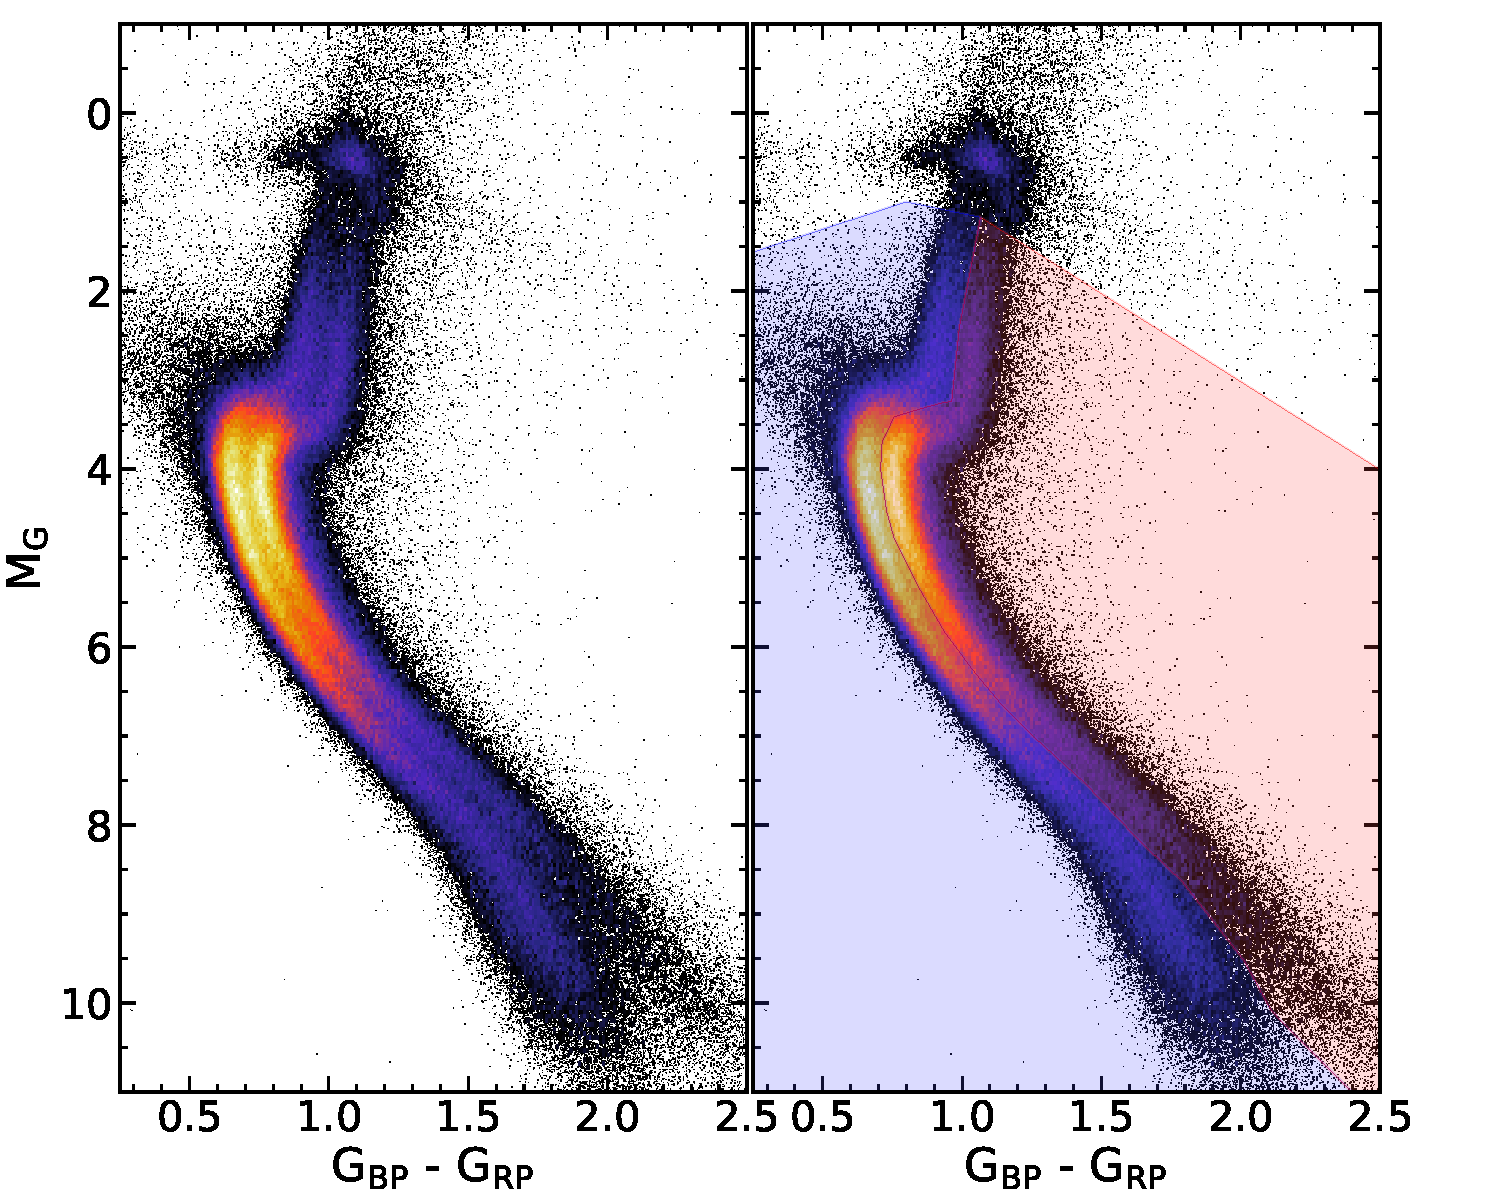
\includegraphics[width=0.75\textwidth]{images/GES_cmd.pdf}
    \caption{Colour-magnitude diagram of our filtered halo sample. Colour shows the number density. Right panel shows selected regions for the left and right sequences overlaid with shaded areas.} % Fig. 5.1
    \label{fig:halo_cmd}
\end{figure}
\begin{figure}[t]
    \centering
    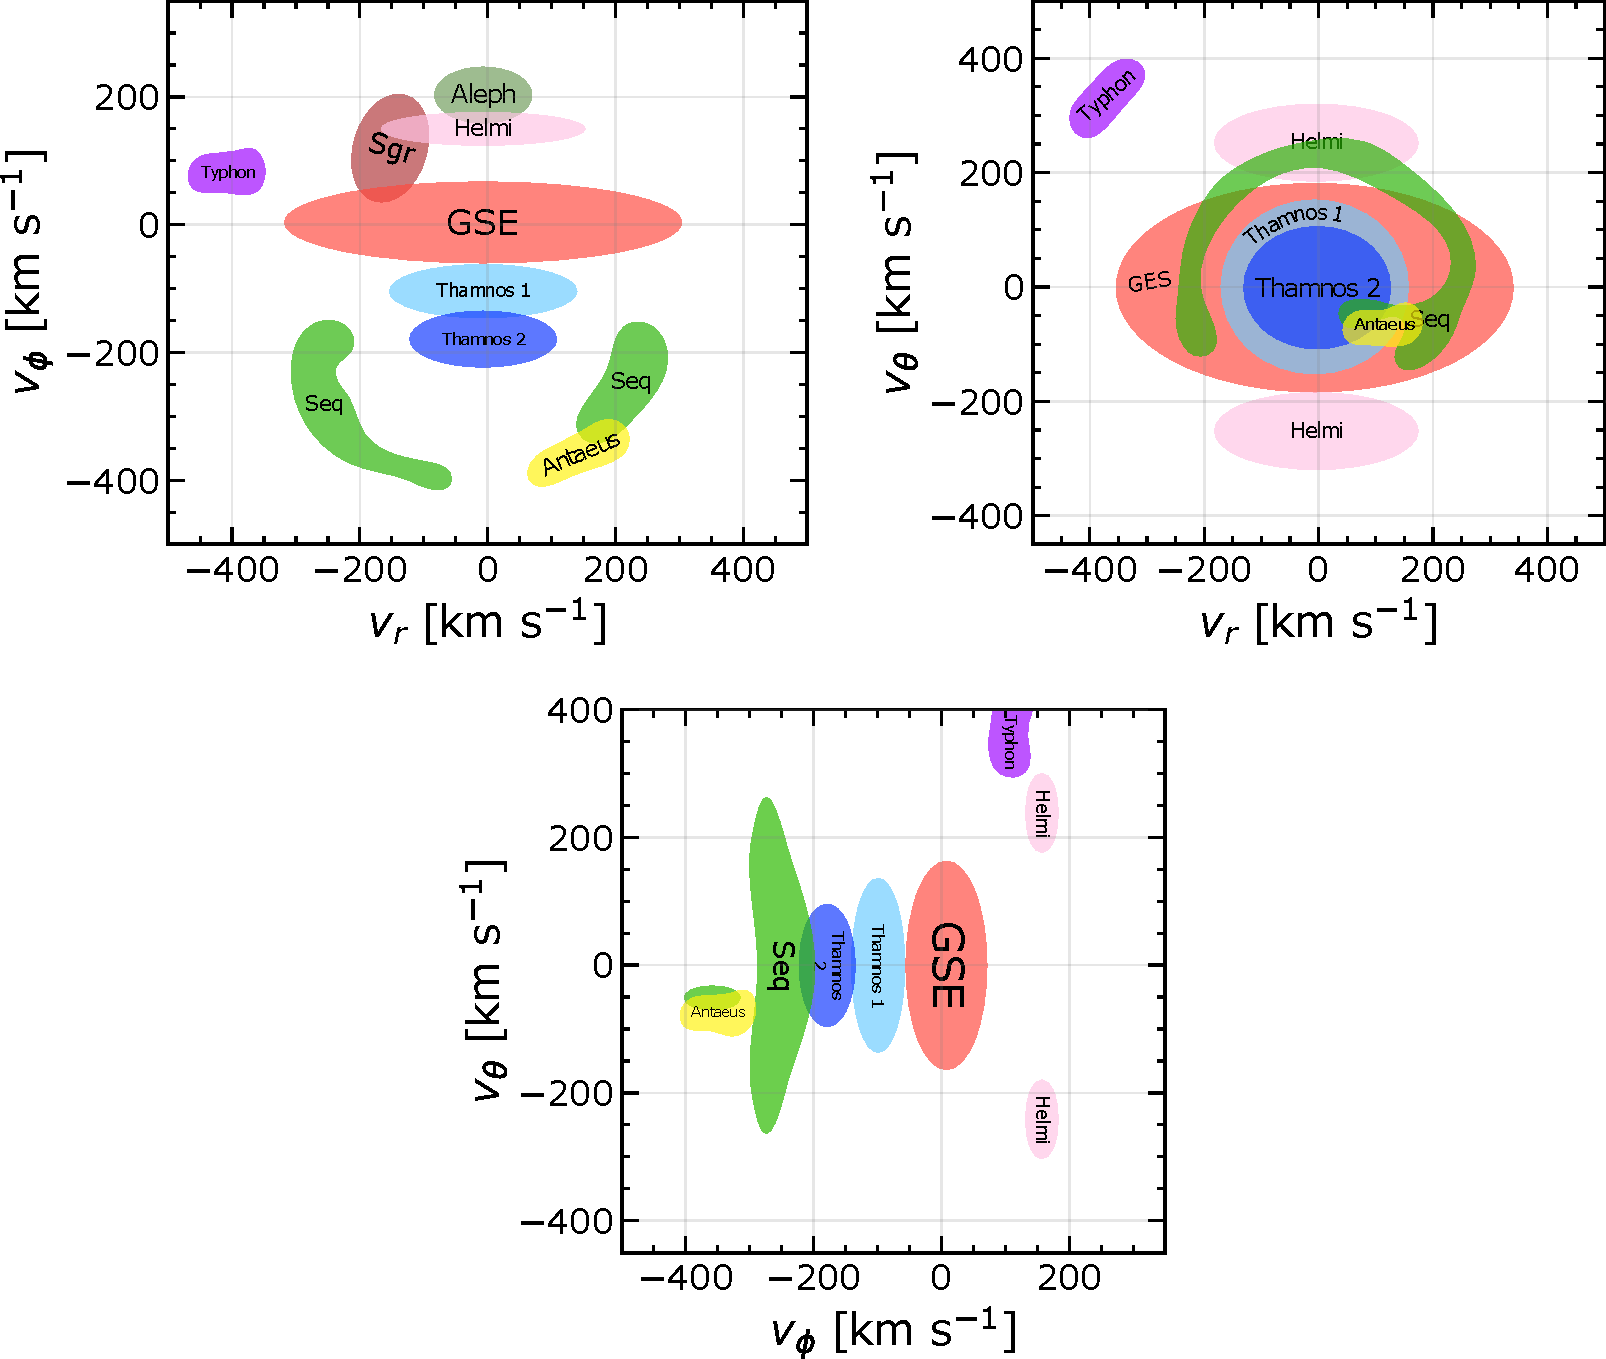
\includegraphics[width=0.85\textwidth]{images/map_only_b.pdf}
    \caption{Estimated typical positions of known velocity structures in the stellar halo. Figures show the velocity spaces of $(v_r, v_\phi)$ (top left), $(v_r, v_\theta)$ (top right), and $(v_\phi, v_\theta)$ (bottom). Here $v_r$ points outwards from the Galactic centre, $v_\phi$ increases in the direction of Galactic rotation, and $v_\theta$ increases from south to north Galactic poles.} % Fig. 5.2
    \label{fig:halo_map}
\end{figure}
There has been plenty of work done to try and characterise the velocity substructure that exists in the disc and stellar halo. We briefly discussed the Solar neighbourhood in chapter \ref{chap:paper2} and showed several moving groups from \cite{antoja:12} in Fig. \ref{fig:wd_fv}. We briefly mentioned \cite{lucchini:22} above which is one of the more recent works that investigates the disc structure. The current picture of the local disc velocity distribution is one with multiple arch-like structures, of which many fractured individual substructures can be identified (see e.g., Table 1 from \citealt{lucchini:22}). 

For the stellar halo, things look slightly different. This is currently a very active field, but some smaller discoveries were made already 20 years ago using Hipparcos to identify the Helmi streams \citep{helmi:99}. It is, perhaps, not surprising that \textit{Gaia} has had a significant impact upon this field as well. When DR2 was released, an important finding for the stellar halo came soon thereafter. By selecting stars with $v_\mathrm{T} > 200$ km s$^{-1}$ \cite{dr2:hr} showed that in the CMD appears two separate main sequences, a finding that we recreate and show in Fig. \ref{fig:halo_cmd}. Rather than a main-sequence with binaries adding a brighter, redder sequence the new sequence appears on the left, consistent with isochrones of a lower metallicity. Based on its kinematics, chemistry, and age the left sequence was found to be connected to an accretion event from a single object \citep{belokurov:18, helmi:18} which is called \textit{Gaia-Sausage-Enceladus} or \textit{GSE}. This lead to a successful hunt for other accreted populations in the stellar halo. This matched very well to the notion of a Galaxy formed through hierarchical growth, suggested by the $\Lambda$CDM model mentioned in Section \ref{subsec:components-stellarhalo}. At the time of writing, some of the larger discovered structures include \textit{Sequoia} \citep{myeong:19}, \textit{Antaeus} \citep{oria:22}, \textit{Thamnos} 1 and 2 \citep{koppelman:19}, and \textit{Typhon} \citep{tenachi:22}, to name a few. We show the expected positions of these features as well as some smaller ones in Fig. \ref{fig:halo_map}. This puts into perspective how structured the Galactic stellar halo has been revealed to be with the use of \textit{Gaia} data.

Since we have access to the most expansive catalogue of sources from \textit{Gaia}, we aim to expand the view of substructure in the local parts of the Galaxy's disc and stellar halo.

\section{Structures: The old and the new}\label{sec:p3-structures}
\begin{figure}[t!]
    \centering
    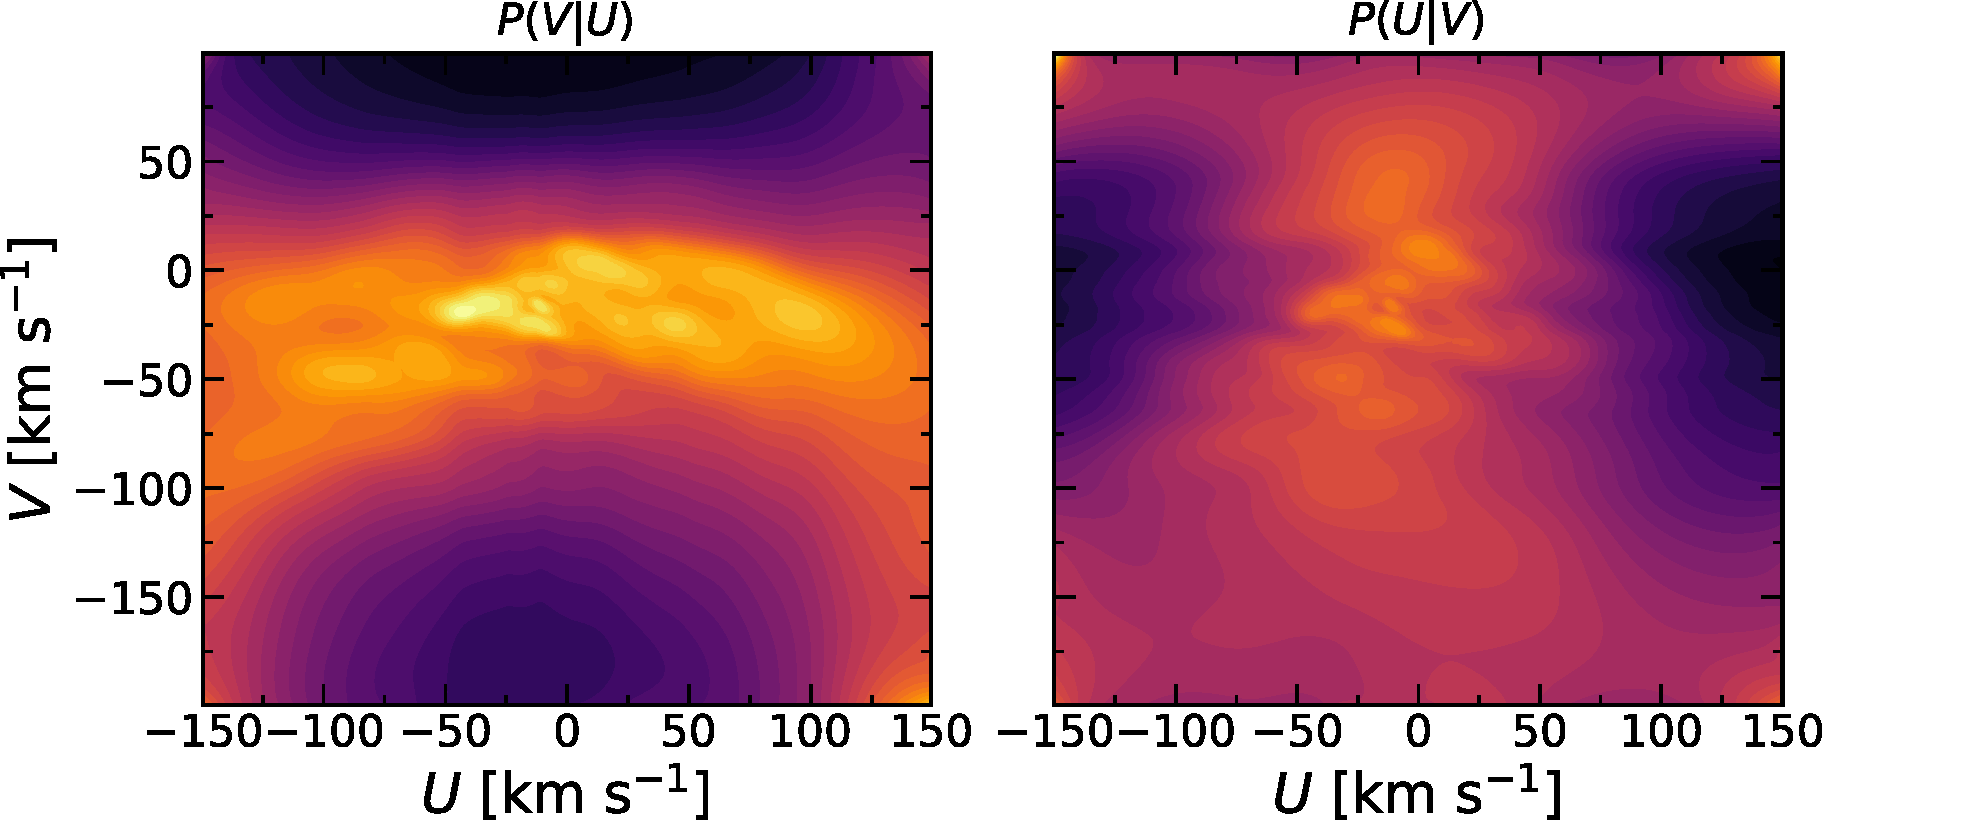
\includegraphics[width=0.9\textwidth]{images/conditional_snbh.pdf}
    \caption{The conditional probability of one velocity component in $(U, V)$ against the other. Left shows $P(V|U)$ and right shows $P(U|V)$ which reveals rich substructure beyond the central dominating groups. The color shows the density scaled as $P(v)^{0.25}$.} % Fig. 5.3
    \label{fig:cond_snbh}
\end{figure}
\begin{figure}[t!]
    \centering
    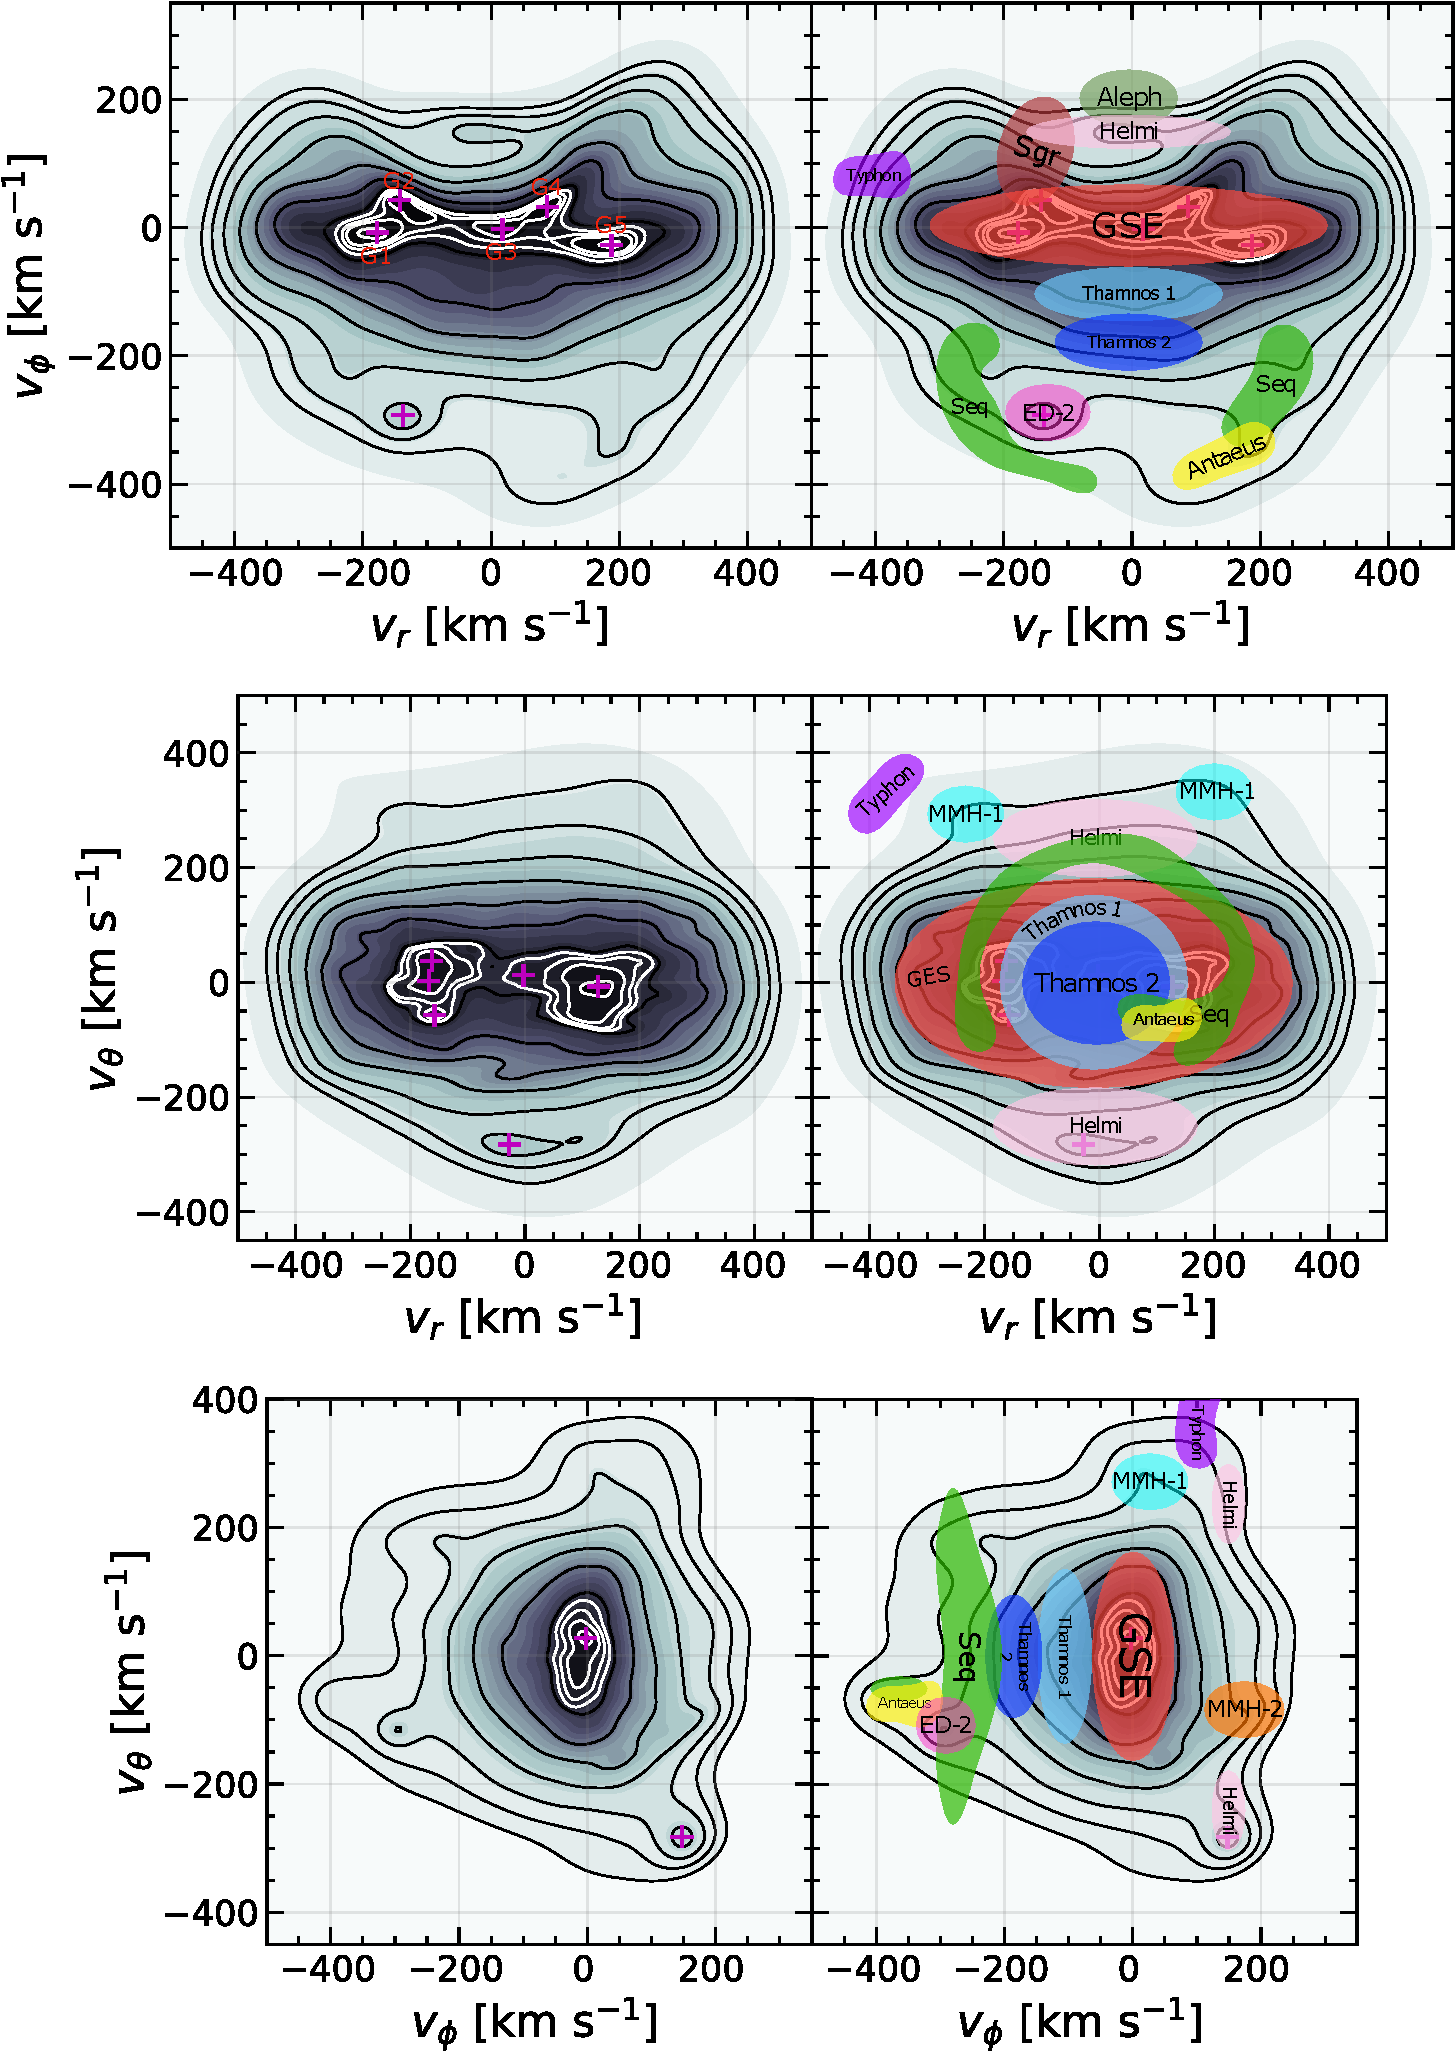
\includegraphics[width=0.8\textwidth]{images/halo_fv.pdf}
    \caption{Velocity distributions of our left halo sample in $(v_r, v_\phi)$ (top row), $(v_r, v_\theta)$ (middle row), and $(v_\phi, v_\theta$ (bottom row). Right right column shows the same distributions overlaid with the positions of expected substructure from literature, in a similar style to what is done in \cite{naidu:20} and \cite{mardini:2022}. Significant peaks are marked with purple crosses and in the top left figure five significant groups belonging to the \textit{GSE} are marked as G1-G5.} % Fig. 5.4
    \label{fig:halo_fv}
\end{figure}
\begin{figure}[t!]
    \centering
    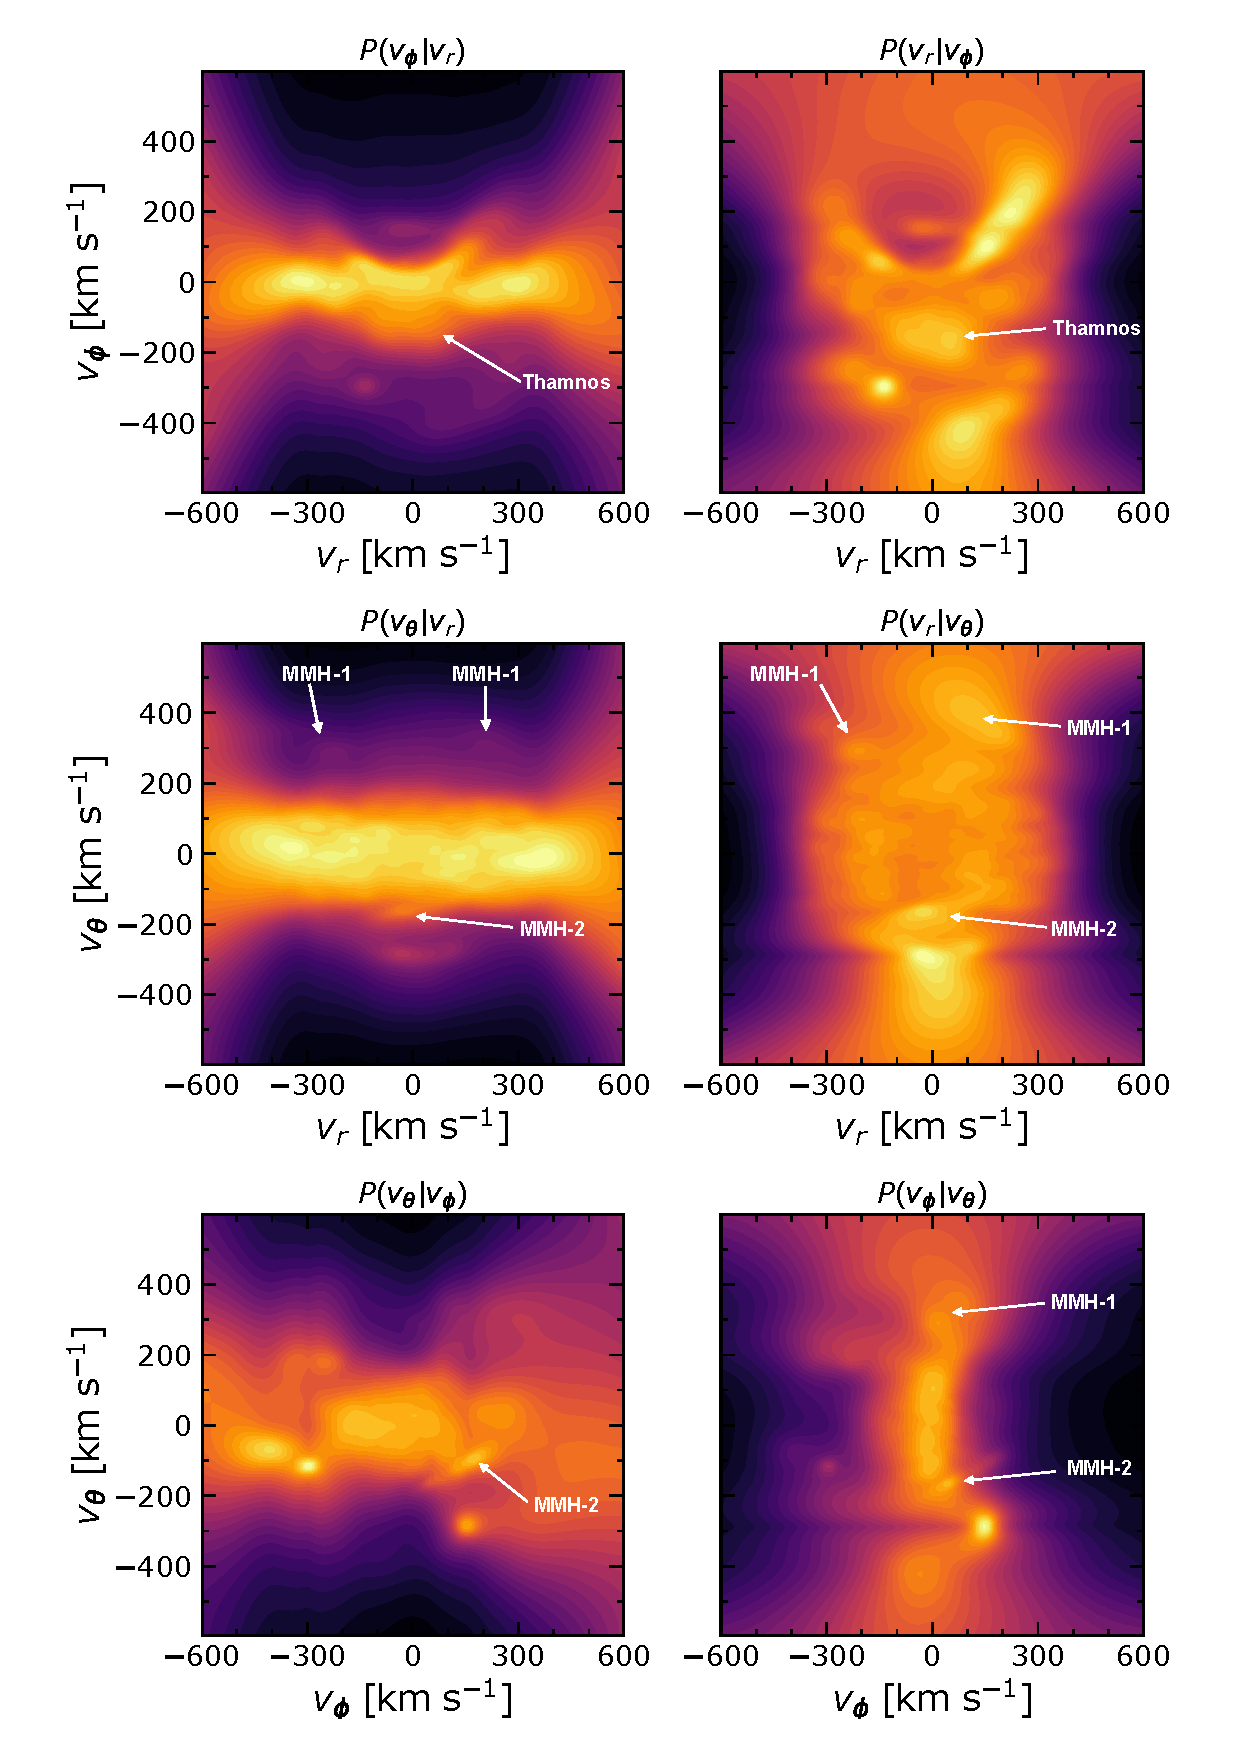
\includegraphics[width=0.75\textwidth]{images/conditional_halo.pdf}
    \caption{Conditional probability distributions of the velocities from Fig. \ref{fig:halo_fv} with the left column showing the conditional probability distribution of the $y$-axis velocity on the $x$-axis velocity. The right column shows the inverted conditional probabilities. Density is scaled as $P(v)^{0.25}$. The arrows show features discussed in Section \ref{sec:p3-structures}. This map is used to unveil further information in the phase-space structure and as such the other features of Fig. \ref{fig:halo_fv} are not labelled here.} % Fig. 5.5
    \label{fig:cond_halo}
\end{figure}
When we investigated the velocity distribution of the Solar neighbourhood we found that the distribution is heavily dominated by the typical major moving groups: \textit{Sirius}, \textit{Coma Berencies}, \textit{Hyades}, \textit{Pleiades}, and \textit{Hercules}. The distributions also contains weaker traces of \textit{Dehnen98} and \textit{Wolf630}. Since the distribution is so heavily dominated by these features, a better way of  unravelling low-level structure that these representations of the velocity distribution may have missed is to renormalize the plots. This implies that rather than showing the full 2D probability density of $U$ and $V$, we show the \emph{conditional} probabilities of $V$ or $U$ for each $U$ or $V$, respectively. That is, the colour represents the probability of the star having a specific $V$ given that it has certain $U$ velocity (or vice versa). The result is probability maps that can reveal structure that is otherwise blotted out by the major groups and we show this in Fig. \ref{fig:cond_snbh}. Here can be seen much richer structure like $\epsilon$\textit{Ind} (e.g., \citealt{antoja:12, kushniruk:17, bobylev:16}) at $(U, V) = (-100, -50)$ km s$^{-1}$, \textit{Dehnen98} \citep{antoja:12} at $(U, V) = (50, -30)$ km s$^{-1}$, and likely \textit{Antoja12} from e.g. \cite{kushniruk:17} at $(U, V) = (100, -30)$ km s$^{-1}$. The conditional probability maps are clearly a useful tool for the outer regions.

The velocity distributions of the two halo samples were determined and as expected, the right sequence shows very little accreted structure and as such we placed most of our focus on the left sequence. The velocity distributions are shown in Fig. \ref{fig:halo_fv} and are overlaid with the expected positions of stellar halo substructure from Fig. \ref{fig:halo_map}. These distributions show clearly a lot of the known velocity substructures such as \textit{GSE}, \textit{Sequoia}, and the \textit{Helmi} streams. Particularly the \textit{GSE} in $(v_r, v_\phi)$ shows a lot of structure with significant peaks marked as G1-G5. The groups at largest $v_r$, 1 and 5, are placed where the \textit{GSE} is typically associated (e.g., \citealt{feuillet:21}). G2 and G4 lie near the region which is removed by our cut of $v_\mathrm{T} < 200$ km s$^{-1}$ and is therefore probably contaminants from  the disc population. Finally G3 matches with Cluster 3 of \cite{lovdal:22} which is also called \textit{L-RL3} in \cite{dodd:22}. The distributions do show some of the smaller features as well and particularly the low $v_\theta$-component of the \textit{Helmi} stream is very pronounced here. These figures give a good impression of what the accreted stellar halo looks like at `face-value'.

Beyond these larger structures, there are a three additional ones that we are able to identify. The first is \textit{ED-2} from \cite{dodd:22} at roughly $(v_r, v_\phi, v_\theta) = (-150, -300, -300)$ km s$^{-1}$. In \cite{dodd:22} they note that it occupies about 0.05\% of their sample with 33 proposed members. This region of velocity space makes up around 0.075\% in our sample, suggesting that the group is slightly larger than previously believed. We are also able to make out two new velocity features which we call \textit{MMH-1} and \textit{MMH-2} which have no prior associations in literature. The first, \textit{MMH-1}, lies at about $(v_r, v_\phi, v_\theta) = (\pm225, 25, 325)$ km s$^{-1}$ and is visible in the spaces of $(v_r, v_\theta)$ and $(v_\phi, v_\theta)$. It is placed in the dense regions in $(v_r, v_\phi)$ and is therefore difficult to spot there. The second is \textit{MMH-2} which is around $(v_\phi, v_\theta) \approx (150, -100)$ km s$^{-1}$ and is difficult to place in the other spaces. However, its $v_r$ component became clear when we again looked to the conditional probability of the velocities, seen in Fig. \ref{fig:cond_halo}. Here, the sloped feature centred around $(v_r, v_\theta) = (0, -125)$ km s$^{-1}$ stands out, and is the representation of \textit{MMH-2} in this space. This shows also that the full extent of \textit{MMH-2} is obscured in Fig. \ref{fig:halo_fv} and that its actual velocities are instead centred on $(v_r, v_\phi, v_\theta) = (0, 150, -125)$ km s$^{-1}$.  These maps also reveal some parts of \textit{Thamnos} at $(v_r, v_\phi) = (0, -200)$ km s$^{-1}$ which could previously not be seen. The extended nature of \textit{MMH-1} at $v_\theta = 300$ km s$^{-1}$ is uncovered as well, stretching to even larger values of $v_\theta$ in both $P(v_r|v_\theta)$ and $P(v_\phi|v_\theta)$ and has what appears to be a symmetrical component at large negative $v_\theta$, which if real would likely imply that this feature has considerable vertical action. This view also shows the strength of \textit{MMH-1} as it appears in both $P(v_\theta|v_\phi)$ and $P(v_\phi|v_\theta)$.

The distributions and the insight into the Galaxy that we gain from them clearly advocate for the benefits of working with pure proper-motion limited catalogues. Until such a time that comparative 6D catalogues are available, these types of methods provide the largest possible data sets for kinematic studies. 

